%!TEX root = ./cikm2016.tex
\section{Experiments on \\ Knowledge Completion}
\label{sec:exp1}

\begin{table}[t]
\centering
\caption{\label{tbl:dataset}Description of datasets. 
Sparsity denotes the ration of valid triples to invalid triples.}
\vskip 0.15in
\begin{tabular}{l | r | r | r | r}
Dataset &  \# rel & \# entities & \# triples & sparsity \\ \hline
Kinship & 26 & 104  & 10,790 & 0.038 \\
UMLS & 49 &135  & 6,752 & 0.008 \\
Nation & 56 & 14  & 2,024 & 0.184 \\
%Wordnet & 11 & 38,696  &123,429 & 7.5e-06\\
%Wordnet(N) & 10 & 836 & 1,766 & 2.5e-04\\
\end{tabular}
\end{table}


\begin{figure}[t]
	\centering
	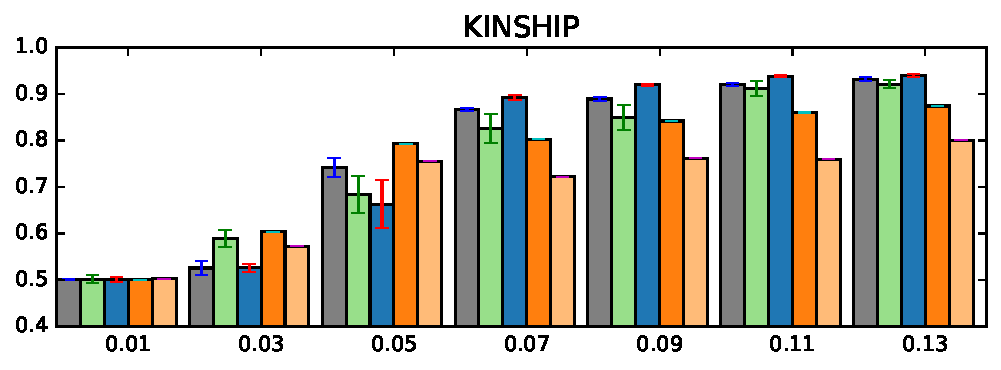
\includegraphics[width=\linewidth]{images/comp_training_error_kinship_small.pdf}
	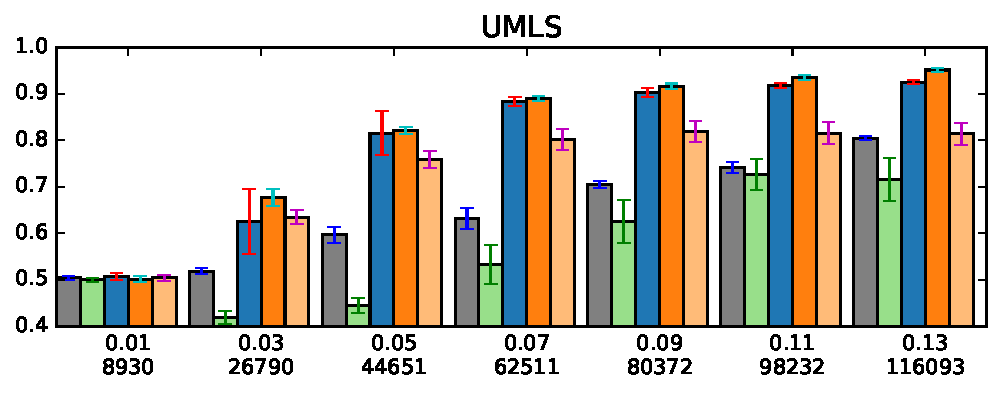
\includegraphics[width=\linewidth]{images/comp_training_error_umls_small.pdf}			
	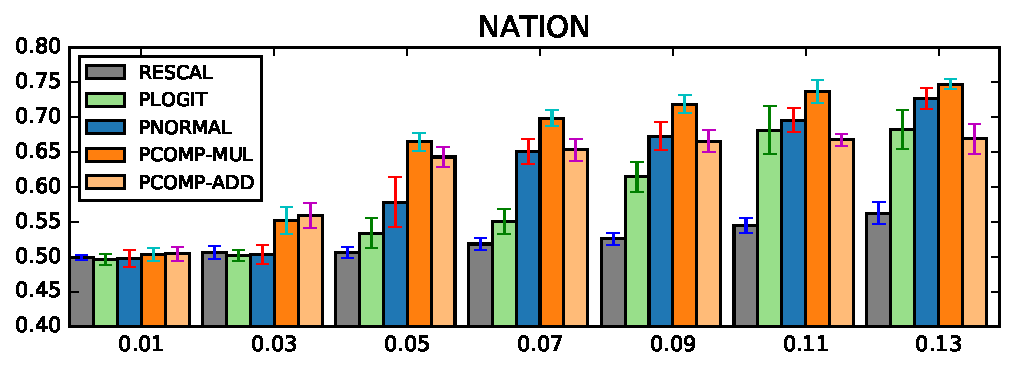
\includegraphics[width=\linewidth]{images/comp_training_error_nation_small.pdf}				
	\caption{\label{fig:r_vs_br} ROC-AUC scores of compositional models. 
	The x-axis denotes the proportion and total number of triples used for training. %We use other 20\% of triples as a validation set and another 30\% of triples as a test set. 
}
\end{figure} 

\begin{figure}[t]
	\centering
	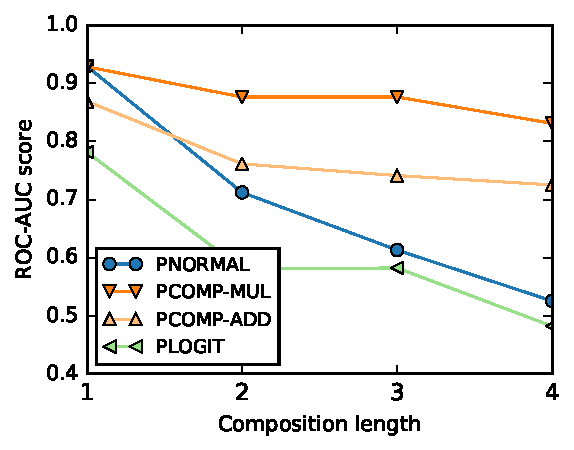
\includegraphics[width=0.7\linewidth]{images/path_prediction2.pdf}
	\caption{\label{fig:path_pred} Path prediction result with UMLS. 
	The performances of both compositional models remain consistent 
	whereas those of the non-compositional models drop sharply as the length increases.}
\end{figure}

\begin{table*}[t]
\center
\small
\caption{\label{tbl:path_example} Example of path prediction from UMLS data. We predict top 5 entities in compositional triples starting from entity \texttt{Mental-or-Behavioral (MB) Dysfunction} followed by two relations \texttt{Affects} and \texttt{Produces}. Correct entities are bolded.}

\subfigure[Triple prediction: \texttt{(MB Dysfunction, Affects, -)}]{
\begin{tabular}{l | p{2.7cm}p{2.7cm}p{2.7cm}p{2.7cm}p{2.7cm}}
Model & Top 1 & Top 2 & Top 3 & Top 4 & Top 5 \\ \hline \hline
PNORMAL & \textbf{Invertebrate}&\textbf{Reptile}&\textbf{Archaeon}&\textbf{Bird}&\textbf{Phy.-Function} \\ \hline
PLOGIT & \textbf{Cell-Function}&\textbf{Disease-or-Syndrome}&\textbf{Cell-or-Molecular-Dysf.}&\textbf{Exp.-Model-of-Disease}&\textbf{Mental-Process} \\ \hline
PCOMP-MUL & \textbf{Archaeon}&\textbf{Fish}&\textbf{Fungus}&\textbf{Invertebrate}&\textbf{Human} \\ \hline
PCOMP-ADD & \textbf{Path.-Function}&\textbf{Bird}&\textbf{Cell-or-Molecular-Dysf.}&Drug-Delivery-Device&Congenital-Abnormality 

\end{tabular}
}
\subfigure[Length-2 path prediction: \texttt{(MB Dysfunction, Affects, Produces, -)}]{
\begin{tabular}{l | p{2.7cm}p{2.7cm}p{2.7cm}p{2.7cm}p{2.7cm}}
Model & Top 1 & Top 2 & Top 3 & Top 4 & Top 5 \\ \hline \hline
PNORMAL & Clinical-Drug&Sign-or-Symptom&Org.-Attribute&Drug-Delivery-Device&Clinical-Attr. \\ \hline
PLOGIT & Amphibian&Gov.-or-Reg.-Activity&Food&Biologic-Func.&Classification\\ \hline
PCOMP-MUL & \textbf{Enzyme}&\textbf{Body-Substance}&\textbf{Biogenic-Amine}&Carbohydrate&\textbf{Immunologic-Factor} \\ \hline
PCOMP-ADD & \textbf{Immunologic-Factor}&\textbf{Body-Substance}&Molecular-Biology-Research-Technique&Clinical-Drug&Chemical-Viewed-Structurally

\end{tabular}
}
\end{table*}

%\begin{figure}[t]
%	\centering
%	\includegraphics[width=\linewidth]{images/path_reconstruction.pdf}
%	\caption{\label{fig:path_pred_example} Example of path-prediction from UMLS. From entity \texttt{Mental-or-Behavioral Dysfunction}, we predict entities after two relations \texttt{Affects}/\texttt{Produces} with different models. Y-axis indicates an ROC-AUC score after each prediction. Labels of x-axis show reachable entities after each relation.}
%\end{figure}

%Applying Thompson sampling to the compositional models is not straight forward. 
%Because, in the compositional model, adding one valid triple in a knowledge base will 
%change the accompanying compositional paths over the extended tensor $\mathcal{X}^L$. 
%Therefore, the system requires to compute potential changes in the 
%compositional structure for every candidate query triple. This computational complexity 
%will increase exponentially as we increase the length of the composition.

%In this experiment, instead running the Thompson sampling for the compositional models,
We first evaluate our model for the knowledge completion task
%we follow the standard train/validation/test approach 
to measure the performance of PRESCAL with all non compositional and compositional variants.
%The results between active acquisition and training and testing are not always coincident, but if the Thompson sampling samples latent features from true posterior of the compositional model, the samples corresponds to the true posterior samples from the training set.

We evaluate the PRESCAL models on three benchmark datasets and compare the performance to various baseline 
algorithms. We use three relational datasets: KINSHIP, UMLS, and NATION. Detailed description of each 
dataset is shown in Table \ref{tbl:dataset} \footnote{https://alchemy.cs.washington.edu/papers/kok07/}.

\begin{figure*}[t]
	\centering
	
	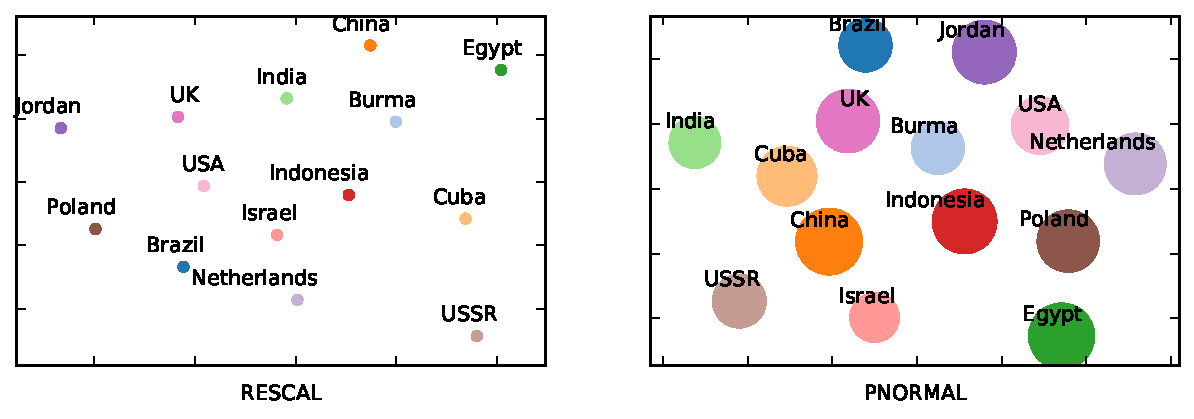
\includegraphics[width=0.7\linewidth]{images/embedding_nation.pdf}

	\caption{\label{fig:tsne} Embedding multi-dimensional entities of the NATION dataset into a two-dimensional space through tSNE \cite{VanDerMaaten2008}. The size of circle in PNORMAL is proportional to the uncertainty of entities in the embedded space. The probabilistic interpretation gives a systematic way to measure the uncertainty of obtained entities.}
\end{figure*}

For all experiments, we set the compositional length $L$ to 2, split the dataset into 20\% for validation and 30\% for testing. We vary the proportion of training triples
from 1\% to 13\% of datasets. For RESCAL, we use the authors' implementation\footnote{https://github.com/mnick/rescal.py}, and measure performance over 10 runs with random initialisations. For PRESCAL and all the variants, we sample triples $x_{ikj}$ from its posterior, and measure performance over 10 different samples.
%Based on the trained model, measure the ROC-AUC scores on the test set.
Given the test set, the performances of models are measured by ROC-AUC score:
\begin{align}
\frac{1}{|\mathcal{X}_p|  |\mathcal{X}_n|} \sum_{\{i,k,j\} \in \mathcal{X}_p, \{i',k',j'\} \in \mathcal{X}_n} \mathbb{I}[\bar{x}_{ikj} > \bar{x}_{ikj}],
\end{align}
where $\mathcal{X}_p$ and $\mathcal{X}_n$ are the set of positive and negative triples in the test set, respectively, and $\bar{x}$ is a reconstructed triple.

Figure \ref{fig:r_vs_br} shows the ROC-AUC scores of the compositional models 
with the various baseline models. We can see that the PRESCAL with 
the normal output (PNORMAL) or logistic output (PLOGIT) generally outperform RESCAL. 
We compare the compositional model with original RESCAL, PNORMAL, and PLOGIT. 
In general, the multiplicative compositional model (PCOMP-MUL) outperforms 
the additive compositional model (PCOMP-ADD), and performs better the other baseline models 
when the proportion of training set is small. For UMLS and NATION, BCOMP-MUL outperforms 
across the all training proportions. 
For KINSHIP, however, the model performs better when the training proportion is less than 7\%.

The goal of the compositional models is to factorise triples along with the graph structure as a whole. 
The triple prediction task tells us the trained model is capable of triple prediction, 
but does not tell whether the features containing the graph structure. 
%Both models perform well in triple prediction, but this does not tell 
If the model factorise the graph structure properly, 
then the trained model can predict not only triples but the graph structure as well. 
To validate the model assumption, we evaluate a path prediction task.
For this task, we use 10\% of UMLS dataset for training. 
We compute the expected value of unobserved compositional triples given a trained model. 
The non-compositional models are not capable to compute the expected value. 
In such case, we approximate the triples with multiplicative model assumption in Equation \ref{eqn:multi}. 
We vary the compositional length from 1 (triple) to 4, and measure ROC-AUC scores on the reconstructed compositional triples. 
Figure \ref{fig:path_pred} shows the result. 
Both compositional models show consistent performance regardless of the compositional length. 
It is worth emphasising that although the compositional length for training is 2, 
the compositional models show consistent results on predicting triples of length 3 and 4. 
Table \ref{tbl:path_example} shows an example of the path prediction result 
starting from entity \texttt{Mental-or-Behavioral (MB) Dysfunction} followed by two relations \texttt{Affects} and \texttt{Produces}. 
Both compositional and non-compositional models predict length-1 triples well. 
With length-2 compositional triples, only the compositional models can capture correct entities on top 5.

We visualise the multi-dimensional entities inferred from RESCAL and PNORMAL of the NATION dataset into a two-dimensional space through tSNE \cite{VanDerMaaten2008} in Figure \ref{fig:tsne}. The probabilistic interpretation gives a systematic way to measure the uncertainty of obtained entities while the RESCAL cannot.
